\startchapter{Sage Archetecture}
\label{chapter:arch}


In this Chapter we take a look at the architecture of SageFS. We first get a high level overview of the entire system, then dive into each component for more details. Finally, we examine some of the missing features of Sage and discuss how they could be introduced into the architecture.

\section{Design Goals}

Sage was originally designed for use on the GENI Experiment Engine (GEE). The GEE allows users to get nodes on a remote network and is designed to be a very easy to use, flexible system for experimenters to quickly run an experiment. As such the filesystem design inherited the same principles, namely simplicity and flexibility. From a simplicity point of view, I wanted Sage to be extremely lightweight and be only a thin layer between an application and the actual backend store.

Although Sage was originally part of the GEE, there is no reason for it to exists strictly in that environment. The first Sage prototype used OpenStack Swift as a backend store. At this time, I discovered I needed to include more than a single Swift site as we were running out of storage space and finding persistent nodes proved challenging. From those observations I decided Sage should be transparent enough to allow users to place files where they choose, as well as add or remove backends on the fly. The design goals for Sage are as follows:

\begin{itemize}
\item Introduce as little overhead as possible compared to directly using a given backend.

\item Be flexible enough to support many diverse backends.

\item Allow users to explicitly place files in backends if they so choose.
\end{itemize}


\section{Overview}

Sage is designed as a client library that abstracts away any given backend stores API into posix like semantics. Applications use the client library to communicate with backend stores and perform file operations. The backend store needs no modifications to communicate with Sage, instead Sage translates filesystem operations into the appropriate set of operations for the backend store through components called translators. As shown in Figure \ref{fig:archetecture} the design of Sage has four layered components:
\begin{itemize}
\item SageFiles, files opened through Sage.
\item SageFS, the central Sage component.
\item Translators, convert Sage operations to backend operations.
\item Backends, existing storage systems.
\end{itemize}

\begin{figure}[h!]
\centering
%keepaspectratio=true, width=\textwidth
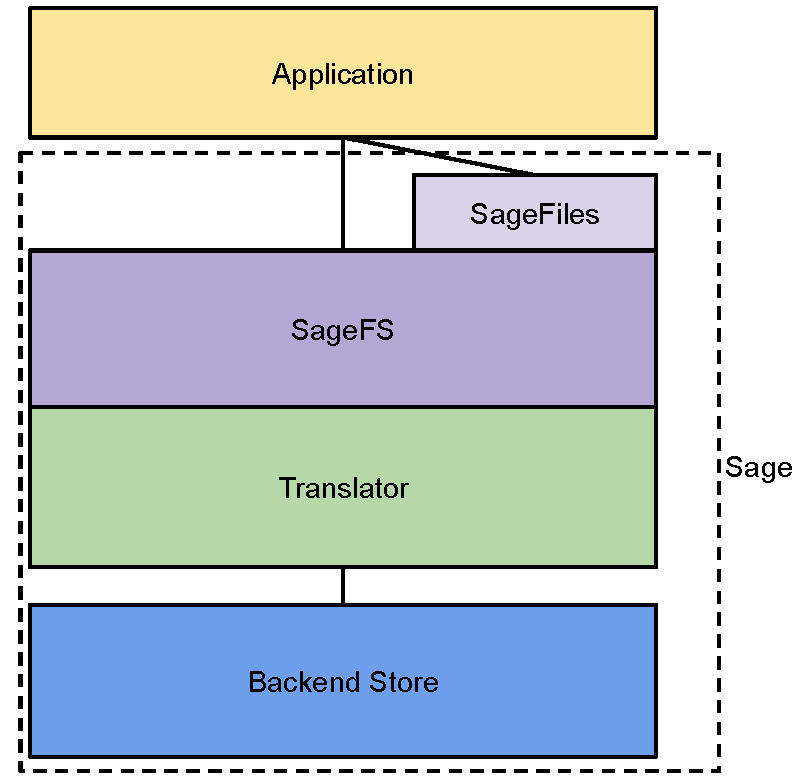
\includegraphics[scale=0.7]{figures/archetecture}
\caption[Sage Archetecture]{Sage Archetecture.}
\label{fig:archetecture}
\end{figure}

An application sees Sage as one filesystem, where within Sage many translators may exist connecting to many different backends. To do this applications interact with SageFS to perform filesystem operations like listing, opening, or removing files, and interact with SageFiles for individual file operations like reading and writing. SageFiles behave exactly like normal files opened normally through the operating system with one exception. They hold Sage specific metadata which allows Sage to place the file in the correct backend using the appropriate translator. SageFiles only interact with SageFS, not translators; this means Sage can move SageFiles between translators without the file knowing. Sage can then move files easily inbetween backends as shown in Figure \ref{fig:sagecommunication}.

SageFS is the only component that interacts with the various translators. Internally SageFS holds a collection of translators. When an application makes a Sage filesystem call, SageFS selects the appropriate translator and forwards the request. This approach lets us define an API for SageFS, which is then implemented by the translators. The Sage API currently contains seven methods open(), remove(), list(), stat(), copy(), move(), and upload(). A translator must implement all seven API calls and convert them into the appropriate set of backend calls. A translator is connected to exactly one backend. The open() call retrieves file data from the connected backend store and returns it in a SageFile. It is also used to create a new file. The remove() call removes file data while list() lists all files present in the backend. stat() returns file metadata such as size, copy() duplicates a files contents, and move() moves a file around in the backend store. The actual implementation by the various currently implemented translators is discussed in Chapter \ref{chapter:imp}.

\begin{figure}[h!]
\centering
%keepaspectratio=true, width=\textwidth
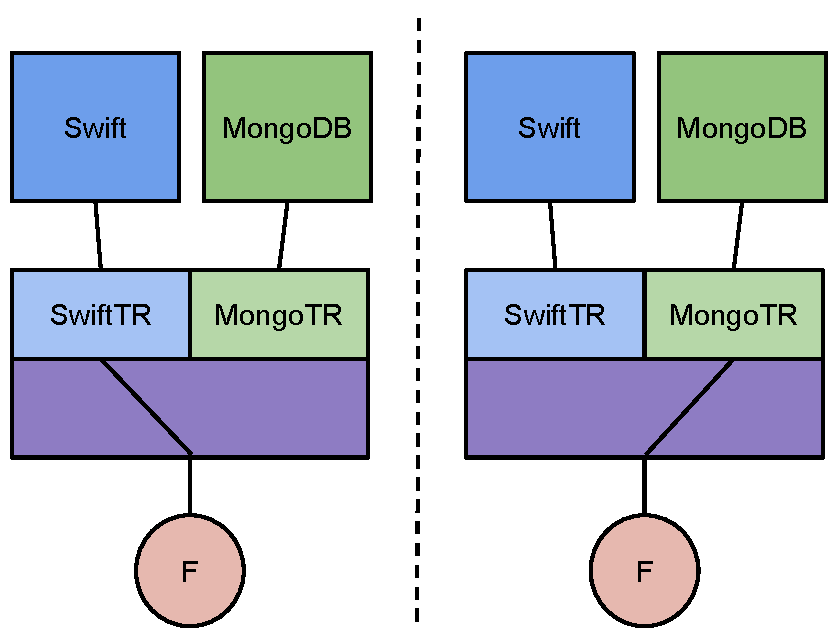
\includegraphics[scale=0.7]{figures/sagecommunication}
\caption[File Interaction in Sage]{File Interaction in Sage. On the left the file F is stored in Swift. SageFS (purple) forwards file requests to the SwiftTR translator. On the right F is stored in MongoDB.}
\label{fig:sagecommunication}
\end{figure}


\section{SageFS}

SageFS creates a common API to many backends systems, but also integrates the backends to look like a single filesystem. SageFS holds a collection of translators that convert filesystem commands into the appropriate set of backend commands. Filesystem commands are performed on paths just like in a posix system, where the root of the path maps to a translator (here we consider \textit{``''} an empty path). For clarity let's examine what happens when an application calls open() on the path \textit{``/vic/test.txt''}. SageFS considers the root to be everything from the leading slash to the second slash of the path, which in this case is \textit{``vic''}. SageFS then maps the root to a translator and calls the translators open with the remaining path, namely \textit{``test.txt''}. Of course, the path could be much larger with many directories. It is the translator's job to map the remaining path to the appropriate data in the backend. In this sense, one of the translator's main functions is to act as a name server for the backend storage service.

List and stat are the only commands that take the empty path as a valid argument. If we look at list, it normally takes a directory as an argument, which prompts SageFS to call the appropriate translators list. However, with no argument SageFS will call list on all the translators it knows about, returning a list of all files within the filesystem. Stat performs the same way.

From the above example it may become clear that Sage knows nothing about which backend files belong to initially. In fact, all file metadata is stored with the backend store. This allows Sage to avoid consistency issues where a backend and Sage disagree on the state of a file. Furthermore, this allows the backend to be manipulated through other channels of operation (not through Sage) without interfering with Sage itself. It also allows multiple Sage instances to connect to the same backends and not have to know about one another. As an aside, all current Sage backends use REST calls to communicate. A backend requiring a constant connection should behave the same way as a REST based one, but this has not been attempted within Sage.

An instance of Sage is a collection of translators that communicate with backend storage services. A single translator talks to a single backend, so if for example we have two backend stores both using Swift, we need two translators one for each Swift instance. We do this as each translator must be independently addressable. If we want to take advantage of each Swift instance independently, we need a way to differentiate between the two. The way Sage holds translators also allows us to add and remove backends by modifying the set of translators in the Sage instance. In fact, when a Sage instance is initially instantiated, the set of translators is empty! It gets populated during operation as backends are addressed. Although more of an implementation detail to reduce initialization time, it demonstrates how resources can be added on the fly to Sage by manipulating the set of translators.

Applications can take advantage of the translator set by explicitly requesting certain backends via the path. By doing this applications can choose where files are placed within Sage. Having control over file placement is beneficial to applications where file location matters, but many applications do not care where their files are placed. Sage can determine file placement if the application does not, and does so through a file placement function. This function takes a full file path and returns a translator within Sage, which is forwarded the request. The default file placement function is primitive. It simply randomly chooses a translator to return, but applications can overwrite the default. Figure \ref{fig:fileplacement} shows the interaction between an application, Sage, and the file placement function. The file placement function can be defined by an application and used to write custom file placement logic.


\begin{figure}[h!]
\centering
%keepaspectratio=true, width=\textwidth
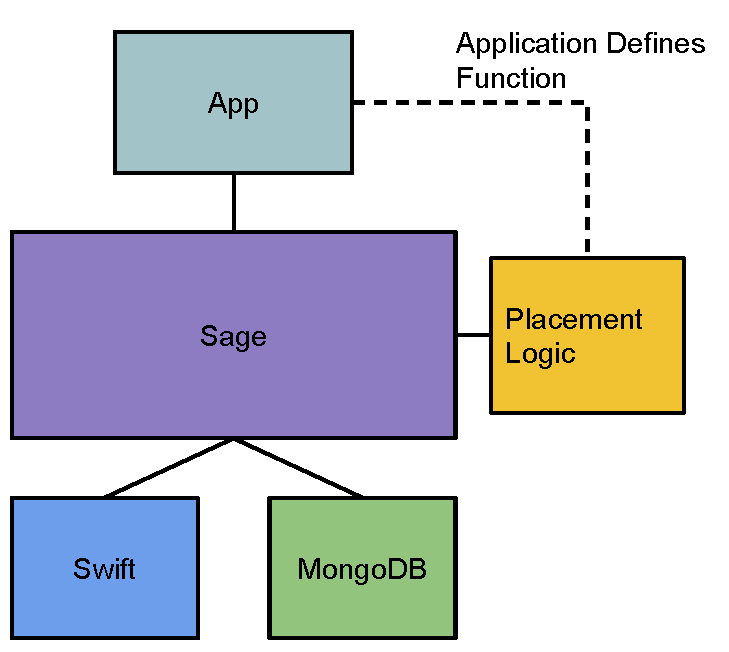
\includegraphics[scale=0.7]{figures/fileplacement}
\caption[Sage File Placement Component]{Sage File Placement Component. Applications can supply a function to overwrite the default file placement logic in Sage.}
\label{fig:fileplacement}
\end{figure}


\section{Filesystem Concepts}

In this section we examine common distributed filesystem concepts, and how they look within Sage.

\subsection{Caching}

Distributed filesystems normally have some form of caching mechanism on clients. Caching helps improve overall performance by providing local copies of resources, so clients do not constantly have to contact storage devices. Sage translators cache file data when a given file is opened within an application. Data is pushed to the backend store when the open file is written to or the closed in Sage. A file is only pulled from the backend when it is opened within Sage, so to revalidate a cached file, the file must first be closed then reopened. More aggressive caching could be performed, where a set of files is kept locally even after they are closed. To do this a timestamp would have to be stored along with the file that could be used to check for staleness by asking the backend store when the cached file was last updated using the stat command.

Sage has no form of cache invalidation. If a stale file is modified on a client and written back to the storage device, the modified stale file will be the authoritative copy of the file. Again Sage could check for timestamps using stat, however a race condition exists here. Suppose we have two clients A and B that want to write a file in the same backend. Client A asks the backend for the time the file was last modified. At the same time Client B asks the backend for a timestamp as well. The backend processes both requests and returns the same timestamp. A and B conclude the file is safe to write when there is a conflict, and the last write will win. This problem comes from a lack of atomicity in the timestamp request. A client can not assume the file has not been modified in the time it takes to get the timestamp from the backend. File locking is normally used to avoid this issue which Sage leaves this up to the backend to handle. If a backend store uses file locking then the translator using the backend will also have file locking, however Sage makes no guarantees about locking in general.


\subsection{File Locking}

As we previously saw, file locking is a way to ensure file consistency with concurrent access. In Sage file locks would either have to be given out by backend stores or each client would have to be aware of each other client and synchronize locking between them. The latter solution is unattractive as clients are allowed to change networks, be behind NAT routers, or perform any other mischief that a traditional network connection would dislike. Furthermore, the filesystem namespace is unique to each client, which would require translation to a common namespace between clients. Moreover, if above problems were not enough of a deterrent the actual locking process would be much worse. 

Clients could hold locks for files but must check first if any other client had a lock on the same file. In the ideal case we, a client, request a file lock and get replies from all others saying they do not have a lock on the specified file. However, what happens if a client does not reply? Do we assume the unresponsive client does or does not have a lock? If the former then we could be waiting for the lock for a while, if the latter then the unresponsive client could assume it has the only lock and commit conflicting changes to the filesystem. Furthermore what if during our lock request we get a request from another client for a lock on the same file. In this case who takes the lock? If we back off and try again (with a random back off or similar strategy), we could potentially get into livelock where we are constantly waiting for locks. This is essentially an instance of the Byzantine Generals problem \cite{Lamport1980,Lamport1983}. Distributed clients must agree on some value (the lock in this case), in an environment with Byzantine failures. Unfortunately, the problem is unsolvable if one-third of the clients fail as consensus requires at least $n/2 + 1$ clients to agree on the value.

Distributed locking is extremely difficult and in fact most distributed lock managers use a central component to avoid such issues. Locking is left to backends in Sage for those reasons. Translators decide how to handle locked files and locks. Since the open call in Sage takes optional arguments locking parameters could be passed into Translators to request locks either blocking or nonblocking. Locks would persist until the file is closed within Sage unless some modification to the API were made, or the application interacted directly with the Translator.

One other issue to consider with locking is Deadlock. Deadlock is a hard issue and normally handled by having locking orders, or by some detection mechanism. Unfortunately in Sage locking orders would be difficult to implement as each client could have a different collection of backends (or the same collection with different names). Hostnames could be used to create a lock order. This way clients get locks from the lexicographically least host first. However, backends can use proxy servers so clients could potentially interact with different hosts to access the same backend. Distributed deadlock detection can be used to track down deadlocks while the system is running by constructing a wait-for-graph \cite{Haas1983}. A wait-for-graph is built between nodes by tracking lock requests and adding edges between nodes that are currently waiting for another. Deadlocks are represented by cycles in the graph. Unfortunately, the graph has to be built at a central component and requires knowledge of all nodes in the system.

Clearly locking poses many problems within the architecture of Sage and is why it is left to the backends. Not only does it simplify the architecture but it also makes Sage more flexible as a system, two key design goals of Sage.


\subsection{Metadata Management}

In Sage metadata is stored with files, much like in a normal filesystem. Filesystem metadata is either stored in the client or queried from the backends. Normally filesystem metadata is stored in a central server, or distributed over a few metadata servers (known as MDSs). With a central MDS, the system has a single point of failure, however with distributed metadata we need to make sure the metadata remains consistent. Sage does not maintain metadata as its flexibility allows backends to be added on the fly which would require a merging of metadata if one were added. Additionally backends can be modified out of band, which could result in files being deleted or modified without the MDS knowing and inconsistencies in the system.


\subsection{Replication}

Replication is usually done in distributed filesystems to improve availability of files. Files are replicated to allow concurrent access,  improve locality, or increase durability. If a file is replicated to multiple copies, updates must propagate to all copies or applications may see inconsistent data (and may modify the inconsistent copy). To enforce consistency systems usually opt for either weak or strong consistency models. Weak or eventual consistency as it is sometimes called guarantees consistency throughout the system eventually. Updates are propagated throughout the system and processed asynchronously by nodes. Operation is not stopped so applications can potentially see stale data if their request is handled before the update. For many applications this is good enough. However some need a better guarantee of consistency. Strong consistency guarantees that once a change is committed, all copies will have the change applied before other applications can access them. This is useful if applications need up to date data, such as a filesystem. It does however impact availability as replicas will be unavailable while a change is being applied.

Keeping the above two schemes in mind Sage could implement replication by assigning replication groups within the client. A replication group is a collection of translators that would perform the same file operations in parallel when one of the members is accessed within Sage. For example, imagine we have a collection of six translators (1 $\dots$ 6). We can set up replication groups as subsets of the translator collection with group size according to the replication factor. With a factor of three we can set up groups (1,2,3), (4,5,6). When a file is accessed through translator 1, it can be read normally, however when changes are made the file is pushed back through translators 2 and 3 as well. This way if translator 1 fails, copies are still on 2 and 3. Updates are done in parallel and should only succeed if updates to all the translators succeed. This is a form of strong consistency as updates are done to all copies and only committed if all replications are updated. There is one caveat here; no file locking is done so it would be possible for two copies to be updated at the same time and writes to overlap differently at different locations. As an illustration assume a file is modified at two places and pushed to the translator group (1,2,3) at the same time. Since last write wins, whichever request is process last is the definitive version of the file. However, each backend could receive modifications in any order and therefore the last update could be different at different nodes. The pushes would succeed, but the file may be inconsistent. Replication groups would have to be the same over all clients or implemented inside translators as clients should know about all replicas of a file to avoid updating only a fraction of the file replicas.

The lack of a dedicated metadata server means replica placement must be computable by a client. Sage could also use hashing to distribute replicas via a consistent hashing algorithm such as CRUSH (previously seen in Chapter \ref{chapter:rel_work}). A filename could be hashed to produce a set of backends to replicate the file to. The set of backends again benefit from being static as adding new backends requires files to be rebalanced to their new hash values. This would involve moving many files between backends, would have to be done by the clients, and cause significant overhead in the filesystem.

\section{Considerations}

Many of the systems currently left to the backends could be implemented if filesystems could not be changed on the fly and were defined for all clients. A static Sage deployment could implement some of the systems discussed. Some design ideas in this chapter could make logical starting points for an implementation, but no prototypes have been developed. The next chapter presents the implementation of Sage. Further discussion of some of the features and ideas presented here are addressed in Chapter \ref{chapter:conc}.